\documentclass[../../../../main.tex]{subfiles}
\begin{document}

\begin{flushright}
\footnotesize\textit{【自動文字起こし・要確認】}
\end{flushright}

\begin{proof}[解]
(i) $f'(x)$ が存在\\
(イ) $x \le 0$ の時 $f(x) = 0$, $1 \le x$ の時 $f(x) = 1$

\begin{center}
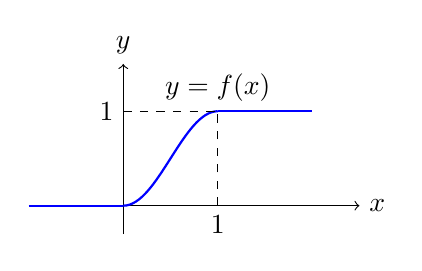
\begin{tikzpicture}[scale=1.2]
  % f(x)
  \draw[->] (-1,0) -- (2.5,0) node[right] {$x$};
  \draw[->] (0,-0.3) -- (0,1.5) node[above] {$y$};
  \draw[thick, blue] (-1,0) -- (0,0);
  \draw[thick, blue] (0,0) cos (0.5,0.5) sin (1,1);
  \draw[thick, blue] (1,1) -- (2,1);
  \node[above] at (1,1) {$y=f(x)$};
  \draw[dashed] (1,0) node[below] {$1$} -- (1,1);
  \draw[dashed] (0,1) node[left] {$1$} -- (1,1);
\end{tikzpicture}
\qquad
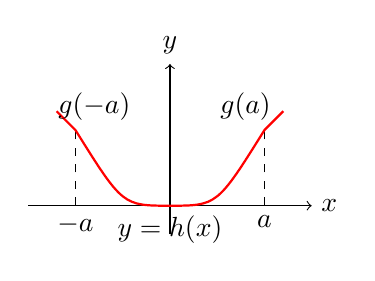
\begin{tikzpicture}[scale=1.2]
  % h(x)
  \draw[->] (-1.5,0) -- (1.5,0) node[right] {$x$};
  \draw[->] (0,-0.3) -- (0,1.5) node[above] {$y$};
  \draw[dashed] (-1,0) node[below] {$-a$} -- (-1,0.8);
  \draw[dashed] (1,0) node[below] {$a$} -- (1,0.8);
  \draw[thick, red] (-1.2,1) -- (-1,0.8) .. controls (-0.5,0) .. (0,0) .. controls (0.5,0) .. (1,0.8) -- (1.2,1);
  \node[above] at (0.8,0.8) {$g(a)$};
  \node[above] at (-0.8,0.8) {$g(-a)$};
  \node[below] at (0,0) {$y=h(x)$};
\end{tikzpicture}
\end{center}

(i) $h(x) = \begin{cases} g(x) f\left(\frac{x}{a}\right) & (0 \le x) \\ g(x) f\left(-\frac{x}{a}\right) & (x \le 0) \end{cases}$ が (イ), (ニ) を満たすことを示す. まず (ロ) から $h(0) = 0$ となって (ハ) を満たす. 次に (ニ) について,
$a < x$ の時 $f\left(\frac{x}{a}\right) = 1$ から $h(x) = g(x)$
$x < -a$ の時 $f\left(-\frac{x}{a}\right) = 1$ から $h(x) = g(x)$
となって (ニ) も満たす. 又 $g, f$ 共に微分可能だから $h(x)$ も $x \ne 0$ では微分可能である. ここで (イ) から $f'(0) = 0$ だから
\[
\lim_{x \to +0} \frac{h(x) - h(0)}{x} = \left. \left( g(x) f\left(\frac{x}{a}\right) \right)' \right|_{x=0} = \left. \left( g'(x) f\left(\frac{x}{a}\right) + \frac{1}{a} g(x) f'\left(\frac{x}{a}\right) \right) \right|_{x=0} = 0
\]
\[
\lim_{x \to -0} \frac{h(x) - h(0)}{x} = \left. \left( g(x) f\left(-\frac{x}{a}\right) \right)' \right|_{x=0} = \left. \left( g'(x) f\left(-\frac{x}{a}\right) - \frac{1}{a} g(x) f'\left(-\frac{x}{a}\right) \right) \right|_{x=0} = 0
\]
となって左右極限が一致し、$x=0$ でも $h(x)$ は微分可能. 以上からこの $h(x)$ は題意を満たす.
\[
h(x) = \begin{cases} g(x) f\left(\frac{x}{a}\right) & (0 \le x) \\ g(x) f\left(-\frac{x}{a}\right) & (x \le 0) \end{cases}
\]

\medskip
(ii) $f(x) = \begin{cases} 0 & (x \le 0) \\ 2x^2 & (0 \le x \le 1/2) \\ -2(x-1)^2 + 1 & (1/2 \le x \le 1) \\ 1 & (1 \le x) \end{cases}$ が (イ) を満たすことをしめす. この関数は全区間で連続である. 又 $x \ne 0, 1/2, 1$ では微分可能.

まず、$g(x) = 2x^2$, $h(x) = -2(x-1)^2 + 1$ とおく. $g'(x) = 4x, h'(x) = -4(x-1)$ であり、
\[
\lim_{x \to +0} f'(x) = g'(0) = 0 = \lim_{x \to -0} f'(x)
\]
\[
\lim_{x \to \frac{1}{2} - 0} f'(x) = h'\left(\frac{1}{2}\right) = 2 = g'\left(\frac{1}{2}\right) = \lim_{x \to \frac{1}{2} + 0} f'(x)
\]
\[
\lim_{x \to 1 - 0} f'(x) = h'(1) = 0 = \lim_{x \to 1 + 0} f'(x)
\]
から、$f(x)$ は $x = 0, 1/2, 1$ でも微分可能. 以上から示された.
\end{proof}

\newpage

\end{document}
